\chapter{Results}
\label{ch:results}

This chapter provides a quantitative and qualitative assessment of our method, by applying it to various scenarios and analysing its output. We begin by formulating a set of odometry and mapping metrics, then observe how our solution behaves if some of its components are altered, and test it on multiple datasets.

\section{Evaluation metrics}
Let us first define the main metrics used for evaluation. In terms of trajectory, Zhang and Scaramuzza \cite{zhang2018tutorial} provide a description of typical metrics for visual odometry, which also apply to LiDAR odometry. Given a ground-truth pose
$\pose_i = \left( \matR_i, \vect_i\right)$ and a corresponding pose
$\widehat{\pose}_i = \left( \widehat{\matR}_i, \widehat{\vect}_i\right)$, we can define translation and rotation errors as:
\begin{equation}
    \begin{aligned}
        e_{\text{trans}}(\vect_i, \widehat{\vect}_i) & = \normtwo{\vect_i- \widehat{\vect}_i} \\
        e_{\text{rot}}(\matR_i, \widehat{\matR}_i )  & = \normtwo{
            \Logmap{\transpose{\widehat{\matR}_i} \matR_i}
        }
        \eqdot
    \end{aligned}
\end{equation}
A simple way to compare two pose sequences that start at the same pose is to compute $e_{\text{trans}}(\vect_N, \widehat{\vect}_N)$ and $e_{\text{rot}}(\matR_N, \widehat{\matR}_N)$, the errors at the final state $N$. A more informative measure is given by the \acrfull{ate} \cite{kummerle2009measuring}:
\begin{equation}
    \begin{aligned}
        \text{ATE}_{\text{trans}} & = \sqrt{\frac{1}{N}\sum_{i=1}^{N} e_{\text{trans}}^2(\vect_i, \widehat{\vect}_i)} \\
        \text{ATE}_{\text{rot}}   & = \sqrt{\frac{1}{N}\sum_{i=1}^{N} e_{\text{rot}}^2(\matR_i, \widehat{\matR}_i )}
        \eqdot
    \end{aligned}
\end{equation}
In the KITTI Benchmark \cite{geiger2012kitti}, this was extended to a metric that is applied on sub-sequences of a certain length or velocity, for a detailed evaluation.

Addressing one of the research questions that motivated this work, we also aim to quantify the quality of the resulting maps, to observe the improvements we bring to the GNSS-merged point cloud. Surprisingly, existing SLAM solutions rarely include rigorous map evaluation, because the map is seen as a localization-enabling tool, rather than a by-product of the system.
The metrics here are closely related to the registration task, but differ in that they are applied on a complete 3D map, instead of a pair of point sets. We note that computing a single value for an entire point cloud is rather misleading, due to variations that appear between its regions, so we aim for point-based metrics that we analyse through a histogram or \acrfull{cdf}.

A high-quality 3D map is expected to be dense, consistent, and provide high detail for observed features. A very trivial metric is the nearest-neighbor distance. Without considering degenerate cases, having a small nearest-neighbor distance is desirable, but this is constrained by the resolution of the sensor --- the distance would be small even when point clouds do not align well, if the LiDAR has high resolution.
Alternatively, we can compute the number of points within a given radius from each point. This is a reliable measure of local density, but it is unable to distinguish between randomly-scattered points and a structured region.
Inspired by the point-to-plane distance (Eq.~\ref{eq:p2plane}), we can compute a metric that measures the deviation of each point from the surface determined by its neighborhood. To avoid noise, we evaluate this for regions that have a high chance of representing planar surfaces, indicated by the normal consistency $c$.
If $\vecx{n}$ and \mbox{$\left\{\vecx{n}_1, \dots \vecx{n}_k\right\}$} are the normals of a point and its neighbors, then
\mbox{$c = \modulus{\transpose{\vecx{n}} \frac{1}{k}\sum_{i \in (1, k)} \vecx{n}_i}$}.

\newcommand{\pk}{\vecx{p}_k}
Another useful metric is given by point entropy, as described in \cite{adolfsson2021coral}. Considering all points within a radius $r$ around point $\pk$, we compute the covariance $\matx{\Sigma}(\pk)$, then derive the differential entropy as:
\begin{equation}
    h(\pk) = \frac{1}{2}\text{ln}\left(
    2\pi e \text{det}\left(\matx{\Sigma}(\pk)\right)
    \right)
\end{equation}
Adjusting the neighborhood radius controls the granularity of the metric, with a value around 0.2m providing a fair trade-off between detail level and computational cost.

To assess computational performance, we provide the processing duration (s) indicating the real time taken for a single input scan, without considering pre-processing operations, when executed on an Intel Core i7-10750H CPU.

% Given a set of ground-truth poses
% \mbox{$\mathcal{T} = \left\{ \pose_i \in \SE{3} : \pose_i = \left( \matR_i, \vect_i\right)\right\}$}, and a corresponding set of predicted poses
% \mbox{$
%         \widehat{\mathcal{T}} = \left\{ \widehat{\pose}_i \in \SE{3} : \right\}
%     $}

% define ATE

\section{Parameter analysis}

In this section we discuss some of the main parameters of our method, in order to better understand their effect on performance, trajectory estimation and final map quality.
\subsection{Point cloud voxelization}
Following the motion compensation applied during dataset pre-processing, every input point cloud undergoes a voxelization step (as described in Section~\ref{subsec:registration}) designed to reduce sensor noise while keeping a sufficient amount of information for registration. We select a subsection of the trajectory consisting of 1000 LiDAR scans and execute the pipeline in LiDAR-only mode (disregarding the GNSS information), with multiple voxel size values. As there are no GPS constraints, the graph optimization step does not modify the pose priors computed by LiDAR odometry. The corresponding GPS trajectory is treated as ground-truth, due to its low uncertainty. The results of this evaluation are presented in Table~\ref{tab:voxel_metrics}. Using a larger voxel size decreases the computational cost, as the point clouds involved have smaller resolution, but introduces considerable problems for odometry estimation, as indicated by the ATE values. We also look at the resulting maps, to confirm that a small voxel size leads to higher-quality mapping, as shown in \reffig{voxel-size-mapping}.

\begin{table}[h]
    \centering
    \begin{tabular}{c|cccccccc}
        \hline
        \textbf{Voxel} & \textbf{Median}   & \textbf{ATE}    & \textbf{ATE}  & \textbf{Final } & \textbf{Final} & \textbf{Avg.} & \textbf{Avg.}   & \textbf{Avg.}  \\
        \textbf{Size}  & \textbf{Duration} & \textbf{Trans.} & \textbf{Rot.} & \textbf{Error}  & \textbf{Error} & \textbf{RMSE} & \textbf{Corr.}  & \textbf{Corr.} \\
                       &                   & \textbf{}       & \textbf{}     & \textbf{Trans.} & \textbf{Rot.}  & \textbf{}     & \textbf{Trans.} & \textbf{Rot.}  \\
        \hline
        \hline
        0.1            & 0.2984            & 1.2814          & 0.0294        & 2.5337          & 0.0467         & 0.0555        & 0.0080          & 0.0010         \\
        0.2            & 0.1684            & 1.3858          & 0.0315        & 2.7607          & 0.0511         & 0.0868        & 0.0210          & 0.0024         \\
        0.3            & 0.1586            & 1.5499          & 0.0347        & 3.0500          & 0.0542         & 0.1206        & 0.0351          & 0.0040         \\
        0.4            & 0.1589            & 1.7736          & 0.0418        & 3.5078          & 0.0659         & 0.1545        & 0.0519          & 0.0055         \\
        0.5            & 0.1603            & 1.4667          & 0.0358        & 2.9164          & 0.0568         & 0.1876        & 0.0819          & 0.0077         \\
        0.6            & 0.1635            & 1.9237          & 0.0475        & 3.7190          & 0.0677         & 0.2186        & 0.1069          & 0.0116         \\
        \hline
    \end{tabular}
    \caption{Metrics for varying voxel sizes. We also show average RMSE values (after registration), alongside the average correction computed by the GICP registration, following the ICP alignment. Translation values are in meters, and rotation values in radians. The duration does not necessarily the voxel size, because more ICP iterations are required for the registration}
    \label{tab:voxel_metrics}
\end{table}

\begin{figure}[h]
    \centering
    \subcaptionbox{Distribution of point entropies.}{
        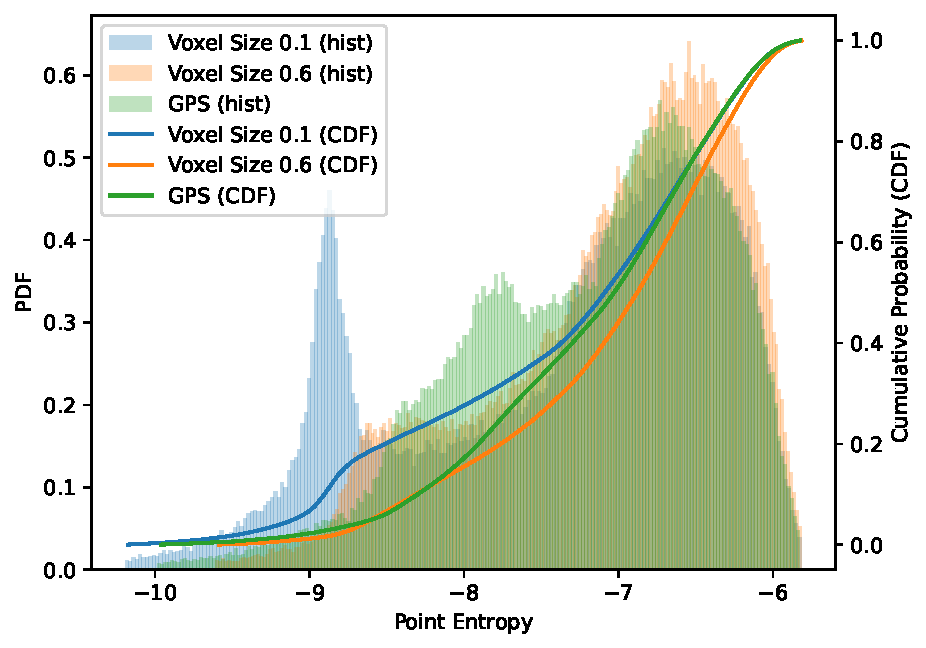
\includegraphics[width=0.45\linewidth]{images/voxel-size-entropy.pdf}
    }
    \hspace{1pt}
    \subcaptionbox{Visual comparison. }{
        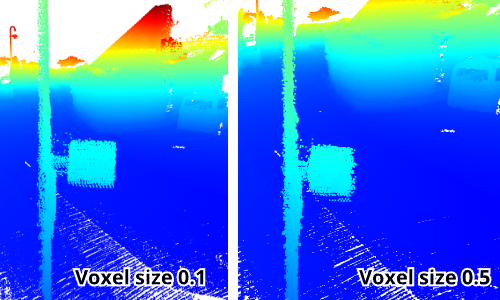
\includegraphics[width=0.47\linewidth]{images/voxel-size-comp.png}
    }
    \caption[Voxel size effect on map quality]{Voxel size effect on map quality.}
    \label{fig:voxel-size-mapping}
\end{figure}



% \begin{figure}[h]
%     \centering
%     \subcaptionbox{Translation corrections.}{
%         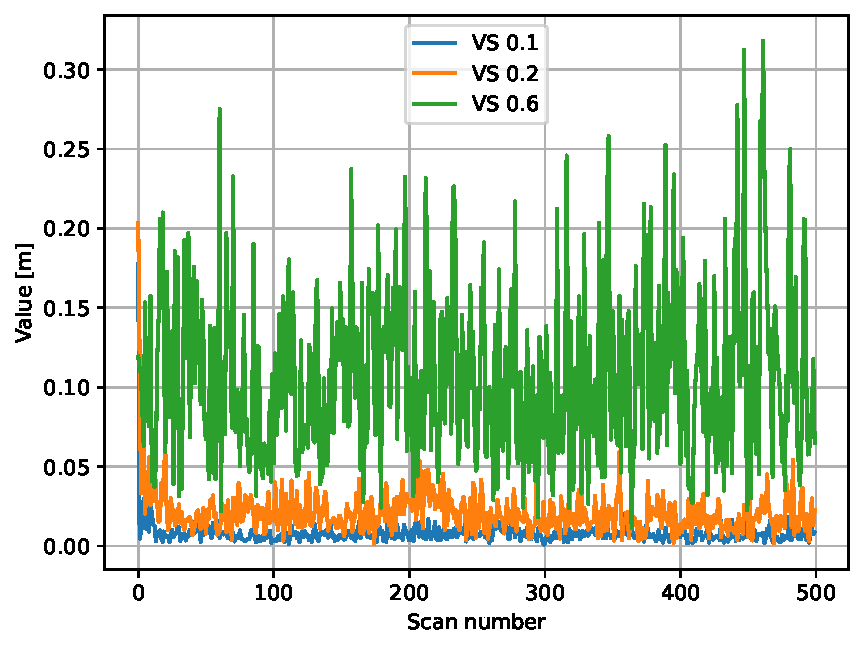
\includegraphics[width=0.46\linewidth]{images/gicp_corrections_trans.pdf}
%     }
%     \hspace{1pt}
%     \subcaptionbox{Rotation corrections.}{
%         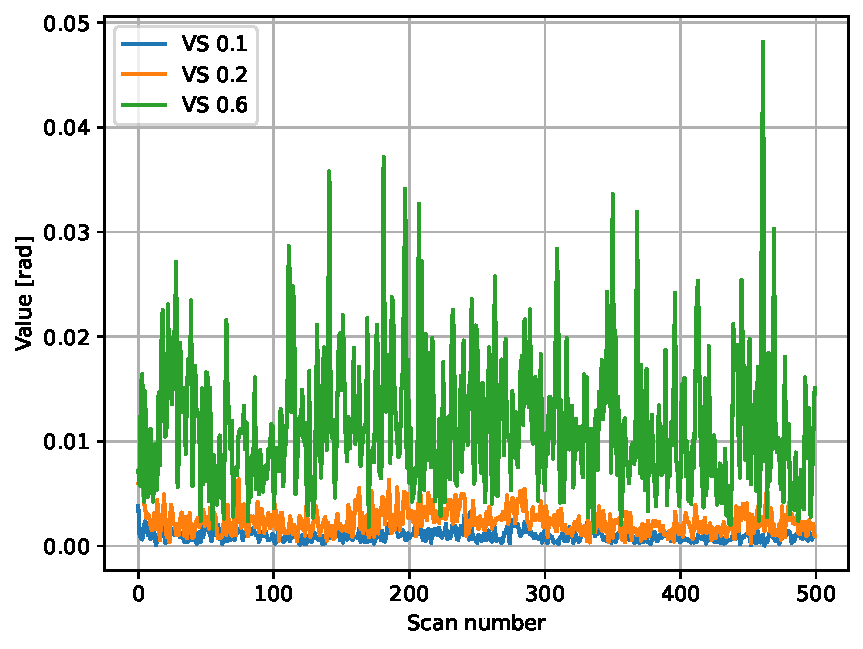
\includegraphics[width=0.45\linewidth]{images/gicp_corrections_rot.pdf}
%     }
%     \caption[]{
%     }
%     \label{fig:gicp-corrections}
% \end{figure}

\subsection{Local map size}
%% how do the results change, depending on the number of previous scans stored

Next, we observe the behavior of the algorithm in relation to the size of the local map, \ie the number of previous scans that the registration is performed against. Given the high frequency and operational range of the sensor, consecutive scans have large overlapping areas which represent useful cues for point cloud alignment. This is proven by the low odometry errors obtained for map size $\geq 5$ in Table~\ref{tab:map_sizes}. As larger maps are used, the computational time increases, but without significant improvements for trajectory estimation.


\begin{table}[h]
    \centering
    \begin{tabular}{c|cccccccc}
        \hline
        \textbf{Map}  & \textbf{Median}   & \textbf{ATE}    & \textbf{ATE}  & \textbf{Final } & \textbf{Final} & \textbf{Avg.} & \textbf{Avg.}   & \textbf{Avg.}  \\
        \textbf{Size} & \textbf{Duration} & \textbf{Trans.} & \textbf{Rot.} & \textbf{Error}  & \textbf{Error} & \textbf{RMSE} & \textbf{Corr.}  & \textbf{Corr.} \\
                      &                   & \textbf{}       & \textbf{}     & \textbf{Trans.} & \textbf{Rot.}  & \textbf{}     & \textbf{Trans.} & \textbf{Rot.}  \\
        \hline \hline
        1             & 0.2349            & 5.0058          & 0.1564        & 10.2891         & 0.2603         & 0.0940        & 0.0366          & 0.0021         \\
        2             & 0.2308            & 4.3812          & 0.1355        & 9.1949          & 0.2318         & 0.0818        & 0.0171          & 0.0016         \\
        5             & 0.2632            & 1.8325          & 0.0458        & 3.6849          & 0.0734         & 0.0615        & 0.0094          & 0.0011         \\
        10            & 0.2962            & 1.2814          & 0.0294        & 2.5337          & 0.0467         & 0.0555        & 0.0080          & 0.0010         \\
        15            & 0.3242            & 1.1645          & 0.0263        & 2.2848          & 0.0415         & 0.0540        & 0.0076          & 0.0010         \\
        25            & 0.3984            & 1.1040          & 0.0245        & 2.1504          & 0.0384         & 0.0531        & 0.0079          & 0.0011         \\
        \hline
    \end{tabular}
    \caption{Metrics for varying map sizes.}
    \label{tab:map_sizes}
\end{table}

\subsection{Registration strategy}
%% how do the results change, depending on whether we use GICP or not

\begin{table}[h]
    \centering
    \begin{tabular}{c|cccccccc}
        \hline
        \textbf{GICP}    & \textbf{Median}   & \textbf{ATE}    & \textbf{ATE}  & \textbf{Final } & \textbf{Final} & \textbf{Avg.} & \textbf{Avg.}   & \textbf{Avg.}  \\
        \textbf{Dist.}   & \textbf{Duration} & \textbf{Trans.} & \textbf{Rot.} & \textbf{Error}  & \textbf{Error} & \textbf{RMSE} & \textbf{Corr.}  & \textbf{Corr.} \\
        \textbf{Thresh.} &                   & \textbf{}       & \textbf{}     & \textbf{Trans.} & \textbf{Rot.}  & \textbf{}     & \textbf{Trans.} & \textbf{Rot.}  \\
        \hline \hline
        -                & 0.2111            & 1.8036          & 0.0371        & 2.8009          & 0.0571         & 0.0601        & -               & -              \\
        0.1              & 0.2949            & 1.1686          & 0.0275        & 1.5486          & 0.0357         & 0.0457        & 0.0070          & 0.0009         \\
        0.2              & 0.3020            & 1.1167          & 0.0280        & 1.4442          & 0.0340         & 0.0520        & 0.0070          & 0.0009         \\
        0.5              & 0.2860            & 1.1958          & 0.0326        & 1.4858          & 0.0390         & 0.0599        & 0.0073          & 0.0010         \\
        \hline
    \end{tabular}
    \caption{Metrics for GICP Variations}
    \label{tab:gicp_variations}
\end{table}

\begin{figure}[h]
    \centering
    \subcaptionbox{Trajectory end point location.}{
        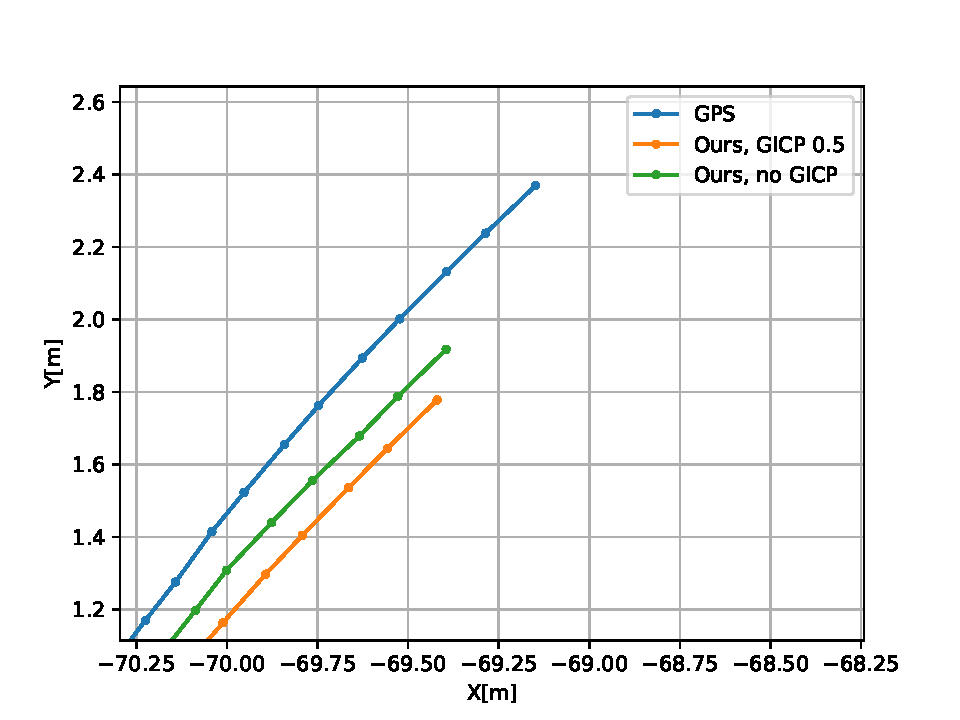
\includegraphics[width=0.46\linewidth]{images/gicp-result-xy.pdf}
    }
    \hspace{1pt}
    \subcaptionbox{Z error evolution.}{
        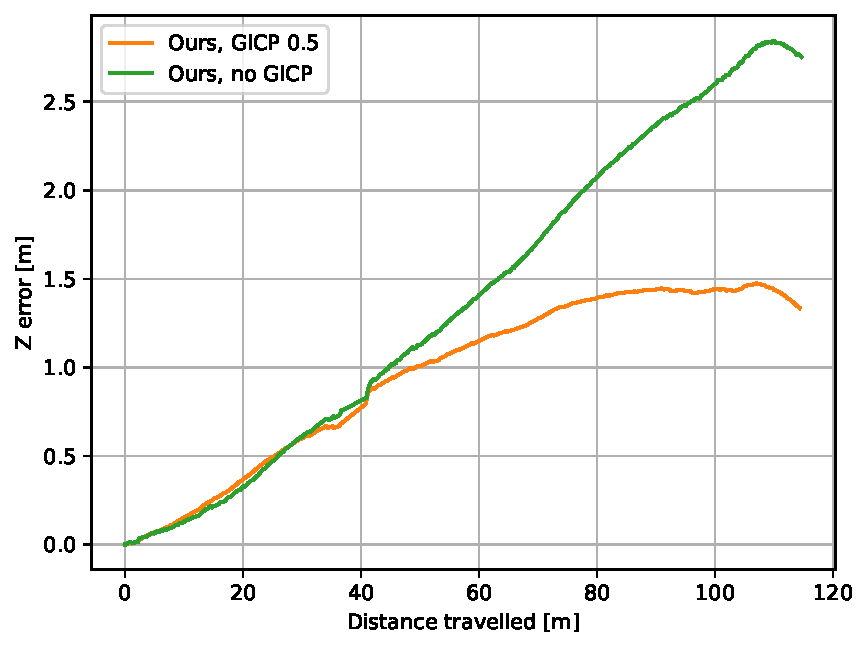
\includegraphics[width=0.45\linewidth]{images/gicp-z-error.pdf}
    }
    \caption[]{
    }
    \label{fig:gicp-traj-result}
\end{figure}

\begin{figure}[h]
    \centering
    \subcaptionbox{Distribution of point entropies.}{
        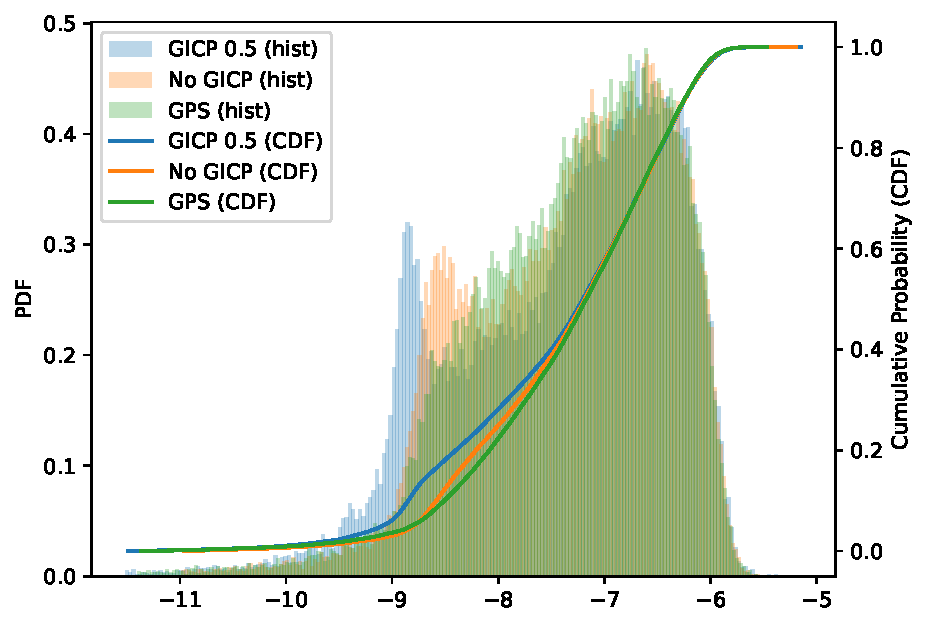
\includegraphics[width=0.46\linewidth]{images/gicp-map-entropy.pdf}
    }
    \hspace{1pt}
    \subcaptionbox{Observing the Z difference in CloudCompare. Yellow - without GICP, white - with GICP.}{
        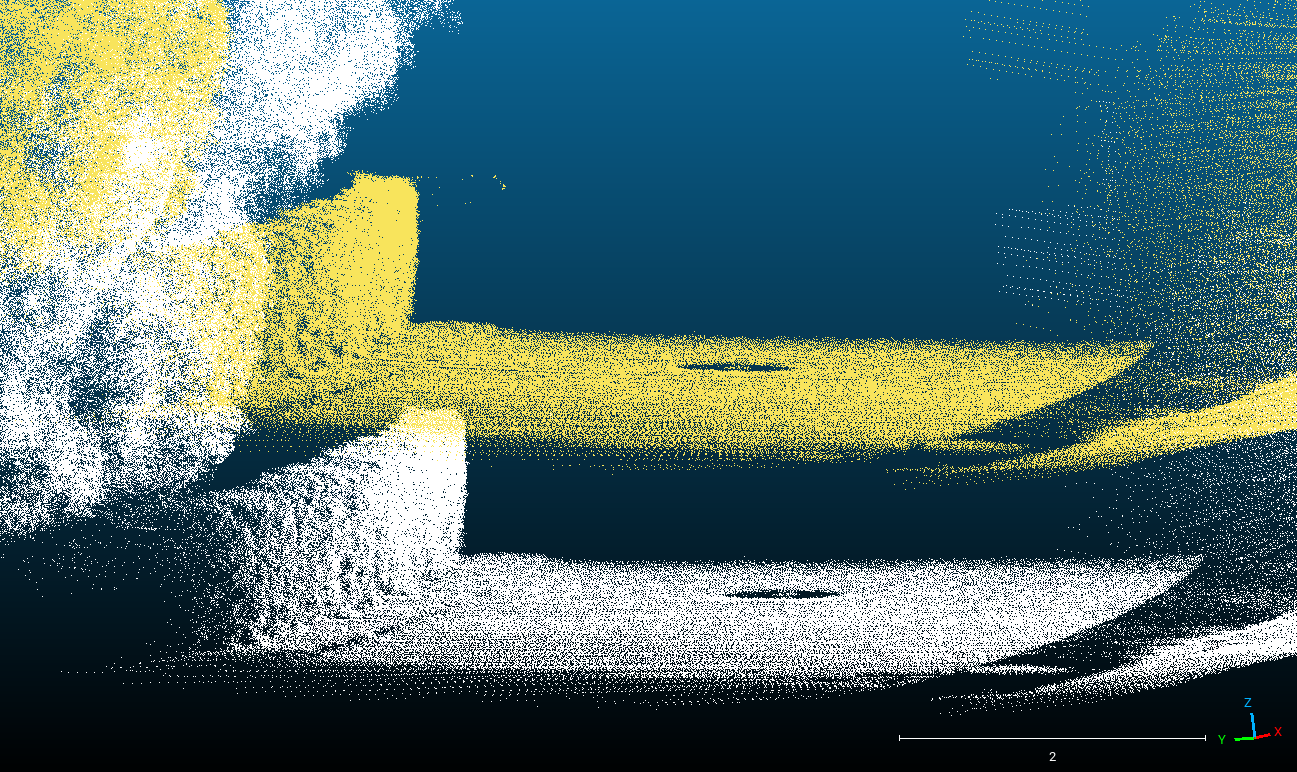
\includegraphics[width=0.45\linewidth]{images/gicp-z-error-view.png}
    }
    \caption[]{
    }
    \label{fig:gicp-map-result}
\end{figure}


\section{Odometry evaluation}

\section{Mapping evaluation}

\section{KITTI results}

% Things worth mentioning
% - execution time